% GeneticWing overview. Build: pdflatex overview.tex, then pdftoppm -png -r 220 -singlefile overview.pdf overview.
% Thumbnails in overview/ are written by scripts/make_flight_gifs.py.
\documentclass[tikz,border=6pt]{standalone}
\usepackage{paperfig}
\begin{document}
\begin{tikzpicture}
% (a) the problem
\node[inner sep=0pt] (sim) {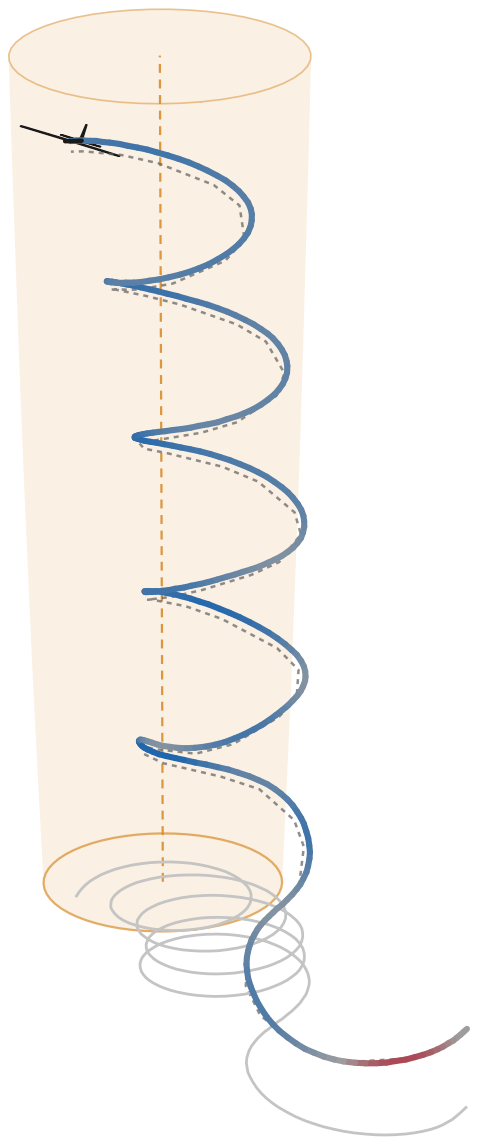
\includegraphics[height=34mm]{overview/flight_thermal.png}};
\node[sub, right=3mm of sim, align=left, anchor=west] (simtxt) {SB-XC\\sailplane\\[2pt]drifting\\thermals\\[2pt]strip wing,\\gusts};

% (b) offline chain
\node[block, text width=23mm, anchor=west] (teacher) at ($(simtxt.east |- sim) + (15mm,0)$)
  {\blocktitle{Teacher}{law + SLSQP\\35 s per plan}};
\node[oursblock, text width=23mm, right=14mm of teacher] (vae) {\blocktitle{Command VAE}{decoder flies\\the commands}};
\node[block, text width=23mm, right=14mm of vae] (ga) {\blocktitle{Latent GA}{3,000 flights\\13 s per plan}};
\node[oursblock, text width=23mm, right=14mm of ga] (gen) {\blocktitle{Generator}{flow matching\\0.24 s per plan}};

% (c) closed-loop flight
\node[thumb, anchor=north west] (xc) at ($(gen.east |- sim.north) + (15mm,0)$)
  {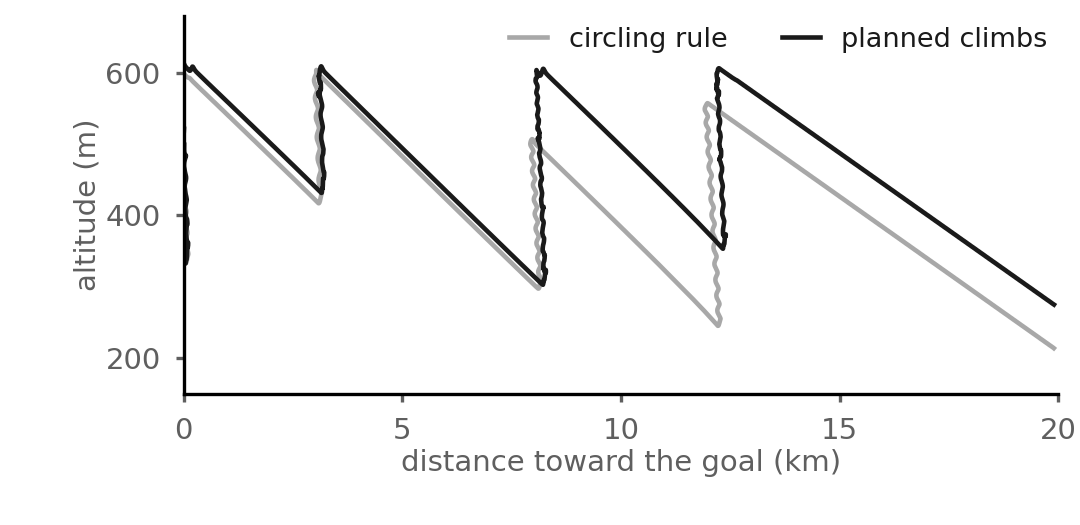
\includegraphics[width=38mm]{overview/flight_xc20km.png}};
\node[keynum, below=1.5mm of xc] (k) {2.23 m/s};
\node[sub, below=0mm of k, align=center] (ktxt) {mean climb, 64 tasks of 20 km\\circling rule: 1.29 m/s};

\draw[flow] (simtxt.east |- teacher) -- node[lab, above, align=center] {climb\\situations} (teacher.west);
\draw[flow] (teacher) -- node[lab, above, align=center] {20,923\\solutions} (vae);
\draw[flow] (vae) -- node[lab, above, align=center] {latent\\$z\in\mathbb{R}^{16}$} (ga);
\draw[flow] (ga) -- node[lab, above, align=center] {best $z$\\per case} (gen);
\draw[flow] (gen.east) -- node[lab, above, align=center] {climb\\plans} (gen.east -| xc.west);

% panels share one height: from the top of the thumbnail to below the headline text
\coordinate (top) at (sim.north);
\coordinate (bot) at ($(ktxt.south |- ktxt.south) + (0,-1mm)$);
\begin{scope}[on background layer]
\node[panelbg, fit=(sim)(simtxt)(sim.north |- bot), inner sep=2.5mm] (pa) {};
\node[panelbg, fit=(teacher.west |- top)(gen.east |- bot), inner sep=2.5mm] (pb) {};
\node[panelbg, fit=(xc)(ktxt)(xc.north |- bot), inner sep=2.5mm] (pc) {};
\end{scope}
\node[paneltitle, anchor=south west] at (pa.north west) {(a) Simulation};
\node[paneltitle, anchor=south west] at (pb.north west) {(b) Offline};
\node[paneltitle, anchor=south west] at (pc.north west) {(c) Closed-loop flight};

% DAgger: the states met in flight go back to the generator
\draw[feedback] (ktxt.south) -- ++(0,-1.5mm) -| node[lab, pos=0.8, left, align=right]
  {DAgger: 1,095 plans\\met in flight} (gen.south);
\end{tikzpicture}
\end{document}
